% cv de Rainan Miranda de Jesus
%Email : Jesus.rainan@gmail.com

\documentclass[margin,line]{res}
\usepackage[utf8]{inputenc}
\usepackage[portuguese]{babel}
\usepackage{graphicx}
\graphicspath{ {assets/} }
\oddsidemargin -.5in
\evensidemargin -.5in
\textwidth=6.0in
\itemsep=0in
\parsep=0in
\usepackage{hyperref}

\hypersetup{
    colorlinks=true,
    linkcolor=blue,
    filecolor=magenta,      
    urlcolor=blue,
    pdfpagemode=FullScreen,
    }

\newenvironment{list1}{
 \begin{list}{\ding{113}}{%
     \setlength{\itemsep}{0in}
     \setlength{\parsep}{0in} \setlength{\parskip}{0in}
     \setlength{\topsep}{0in} \setlength{\partopsep}{0in}
     \setlength{\leftmargin}{0.17in}}}{\end{list}}
\newenvironment{list2}{
 \begin{list}{$\bullet$}{%
     \setlength{\itemsep}{0in}
     \setlength{\parsep}{0in} \setlength{\parskip}{0in}
     \setlength{\topsep}{0in} \setlength{\partopsep}{0in}
     \setlength{\leftmargin}{0.2in}}}{\end{list}}

\begin{document}

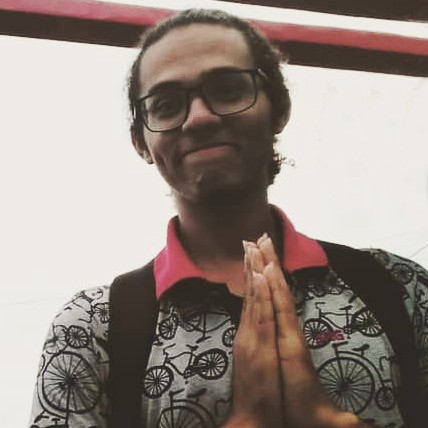
\includegraphics[scale=1.2]{profile.jpg}
\name{Rainan Miranda de Jesus \vspace{0.2cm} \vspace*{.1in}}
\vspace{0.2cm}
\begin{resume}
\section{Informações Pessoais}
\vspace{.05in}
\begin{tabular}{@{}p{2.5in}p{3.5in}}
{\it Endereço: }                   & {\it Data de Nasc.:}  09/10/1996 \\
Av. Oeste, QD 19 LT 24 & {\it Telefone:}  (71) 98691-0699 \\
Camaçari, BA            & {\it E-mail:}  \href{mailto:rainan.jesus@pm.me}{rainan.jesus@pm.me}\\
Brasil                      & {\it }\\
{\it GitHub:}  & {\it LinkedIn:} \\
\href{https://github.com/rainanDeveloper}{rainanDeveloper} & \href{https://www.linkedin.com/in/rainan-miranda-de-jesus-508a43153/}{Rainan Miranda de Jesus}
\end{tabular}
\vspace{0.2cm}
\section{Educação}
\begin{list2}

\item Curso Técnico em Informática no IFBA Campus Camaçari, término em junho de 2018.
\end{list2}
\vspace{0.2cm}
\section{Formação Complementar}
\begin{list2}
\item Minicurso de pre-cálculo
\end{list2}
\vspace{0.2cm}
\section{Conquistas}
\begin{list2}
\item Criação do site de Graduação em computação no IFBA Campus Camaçari
\item Desenvolvimento de aplicação RESTFULL de loja virtual clarion pedido
\end{list2}
\vspace{1cm}
\section{Participação em Conferências}
\begin{list2}
\item Ministrou o minicurso "Programando em PHP", em abril de 2018.
\end{list2}
\vspace{0.2cm}
\section{Experiência}
\begin{list2}
\item Estagiário na IPEM (Inovações Pedagógicas Educação maior), onde era responsável por social media, edição de vídeos, manutenção do site e da rede de computadores. Duração: meses.

\item Estagiário no IFBA Campus Camaçari, onde foi responsável pela criação do site da Graduação em Computação. Duração: meses.

\item Desenvolvedor Júnior FullStack na Clariontec Sistemas - Contratação CLT. Início: 12/2019, até o presente momento.
\end{list2}
\vspace{0.2cm}
\section{Idiomas}
\begin{list2}
\item Inglês - Compreende Bem, Fala Razoavelmente, Lê Bem, Escreve Bem.
\end{list2}
\vspace{0.2cm}
\section{Habilidades Computacionais}
\begin{list2}
\item Linguagens: C, PHP, Python, Javascript ES6, C\#, Java, \LaTeX.
\item Frameworks: ReactJS, React Native, NextJS
\item Tecnologias: NodeJS
\item Amplo conhecimento de Redes, adquiridas no curso técnico.
\item Sistemas Operacionais: Linux, Windows.
\end{list2}
\end{resume}
\end{document}